\documentclass{article}
\usepackage{graphicx}
\usepackage{color}
\usepackage{amsfonts}
\usepackage{fullpage}
\newcommand{\algorithmicbreak}{$\qquad \,\,$ \textbf{break}}
\newcommand{\Break}{\State \algorithmicbreak}
\newcommand{\algorithmictry}{\textbf{try}}
\newcommand{\Try}{\State \algorithmictry}
\newcommand{\algorithmiccatch}{\textbf{catch}}
\newcommand{\Catch}{\State \algorithmiccatch}
\usepackage{subcaption}
\usepackage{times}  
\usepackage{helvet}  
\usepackage{courier}  
\usepackage{url}  
\usepackage{amsmath}
\usepackage{amsthm}
\usepackage{nameref}
\usepackage{varioref}
\usepackage{cleveref}
\usepackage{wrapfig}
\frenchspacing  
\usepackage{color}
\usepackage{comment}
\usepackage{todonotes}
\DeclareMathOperator{\taylor}{Taylor}
\newtheorem{theorem}{Theorem}
\newtheorem{lemma}[theorem]{Lemma}
\newtheorem{proposition}[theorem]{Proposition}
\newtheorem{corollary}[theorem]{Corollary}
\theoremstyle{definition}
\newtheorem{definition}[]{Definition}
\newtheorem{question}[]{Question}
\newtheorem{example}[]{Example}
\newtheorem{remark}[]{Remark}
\newtheorem{assumption}{Assumption}

\usepackage[vlined,ruled,linesnumbered]{algorithm2e}
\usepackage[noend]{algpseudocode}

\newcommand{\argmin}{\mathrm{argmin}}

\usepackage{todonotes}
\usepackage{lineno}

\title{CSE257 Winter 2023: Assignment 3}
\author{}
\date{}

\begin{document}
\maketitle
\linenumbers
Deadline: Mar-5 23:59 PT. 
\begin{itemize}
    \item Submit answer pdf file on Gradescope. Whenever a question asks you to ``Show/Write/List/Plot/Explain" something, you need to include the answers in this pdf file. 
    \item Submit all code as a zip file to \url{https://www.dropbox.com/request/NKRgJpZIlxo0dMVrXea4}.  
\end{itemize}
All other requirements are the same as previous assignments. {\color{red}\bf When a question asks you to plot/show something, you need to show them in the answer pdf. Otherwise points will be taken off.}

\section{Tic-Tac-Toe (Implementation Required)}

Consider Tic-Tac-Toe. I assume you know the rules of the game (type it in Google and play). Now imagine that you are playing it against a purely random opponent. That is, when the opponent needs to make a move, it will choose uniformly randomly from the empty spots, and put its mark in it. We let the opponent plays first: from the empty 9 spots, it first picks an arbitrary one and marks it at the beginning of the game, and then it is your turn. 

Naturally, the game can be modeled as an MDP, with you taking actions from relevant states in the game, and the opponent acting as the environment. Use the following reward function: 
\begin{itemize}
    \item For any game state $s$ that is not terminal (i.e., no winner and there are still empty spots), you receive $R(s)=1$. 
    \item At any game state $s$ where you are the winner, $R(s)=10$, and if you are the loser, then $R(s)=-10$. 
    \item If it is a draw state (all spots are occupied and there is no winner), then $R(s)=0$. 
\end{itemize}
The discount factor is always set to $\gamma=0.9$. 

\begin{figure}[h]
    \centering
    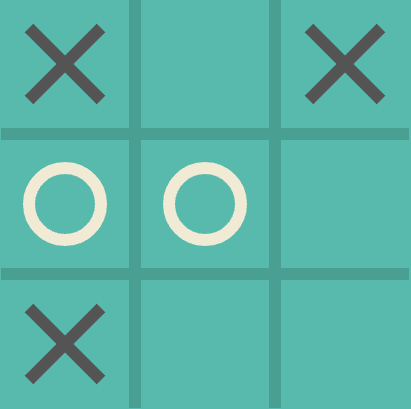
\includegraphics[width=0.3\textwidth]{tic-tac-toe.png}
    \caption{Example of a feasible game state. Your play circle, and it is your turn now.}
    \label{fig:my_label}
\end{figure}

\begin{question}[2 Points]
Implement a random trajectory generator for the MDP that models the game from the perspective of the player (the random opponent and the game rules form the environment). 
That is, given an arbitrary feasible state $s_0$ for the player, generate a random feasible trajectory in the game (of non-zero probability): $s_0,...,s_T$ where $s_T$ is some terminal state. We say a game state is feasible if according to the game rules it is one where the player can take an action, or it is a terminal state. You can assume that your trajectory generator will only be given feasible states as inputs. 

When generating trajectories, in each transition in the sequence, from $s_i$ to $s_{i+1}$, for now you can pick an arbitrary action $a_i$ for $s_i$, and then you need to sample the next state $s_{i+1}$ according to the transition probability $P(s_{i+1}|s_{i},a_{i})$ that is appropriate for the game and the behavior of the random opponent. 

In your answer pdf, list 5 different trajectories generated from different feasible states for the player. Each trajectory that you list should contain more than 2 states. For each trajectory, print the following
\begin{itemize}
    \item The state sequences in the trajectory.
    \item The action and transition probability for each consecutive pair of states. 
    \item The reward-to-go of each state in the trajectory.
\end{itemize}
\end{question}

\begin{question}[3 Points]
Implement value iteration for the MDP, starting from arbitrary initial values of your choice, until the value of every state is at most $0.1$ away from the optimal values (i.e., $\|V-V^*\|_{\infty}\leq 0.1$). 

In your answer pdf, for the game state shown in Figure 1, plot how the value of this particular state changes through the process of value iteration. The x-axis should be the number of iterations, and the y-axis should be its value (some real number). 
\end{question}

\begin{question}[1 Point]
Explain how you know that the value of every state is at most $0.1$ away from the optimal value of that state. 
\end{question}

\begin{question}[1 Point]
For all states that are visited in the 5 trajectories that you listed in the first question, list their optimal values in your answer pdf. Also list the optimal action for each non-terminal state in those trajectories. 
\end{question}

\begin{question}[2 Points]
Pick an arbitrary one of the initial states in the 5 trajectories you showed. Say this is state $s$. Generate $100$ random trajectories from $s$, where the actions for every state in the trajectories are fixed to be optimal actions that you found after value iteration. For $k\in [1,100]$, plot the average reward-to-go $G(s)$ of $s$ in the first $k$ trajectories. i.e., $\frac{1}{k}\sum_{i=1}^k G(s)$ as a function over $k$ (check slides for the mathematical definition of $G(s)$). In the plot, the x-axis should be $k$ and the y-axis is the average reward-to-go. 
\end{question}



\section{Avoiding Pedestrians (Implementation Required)}

\begin{figure}[h!]
    \centering
    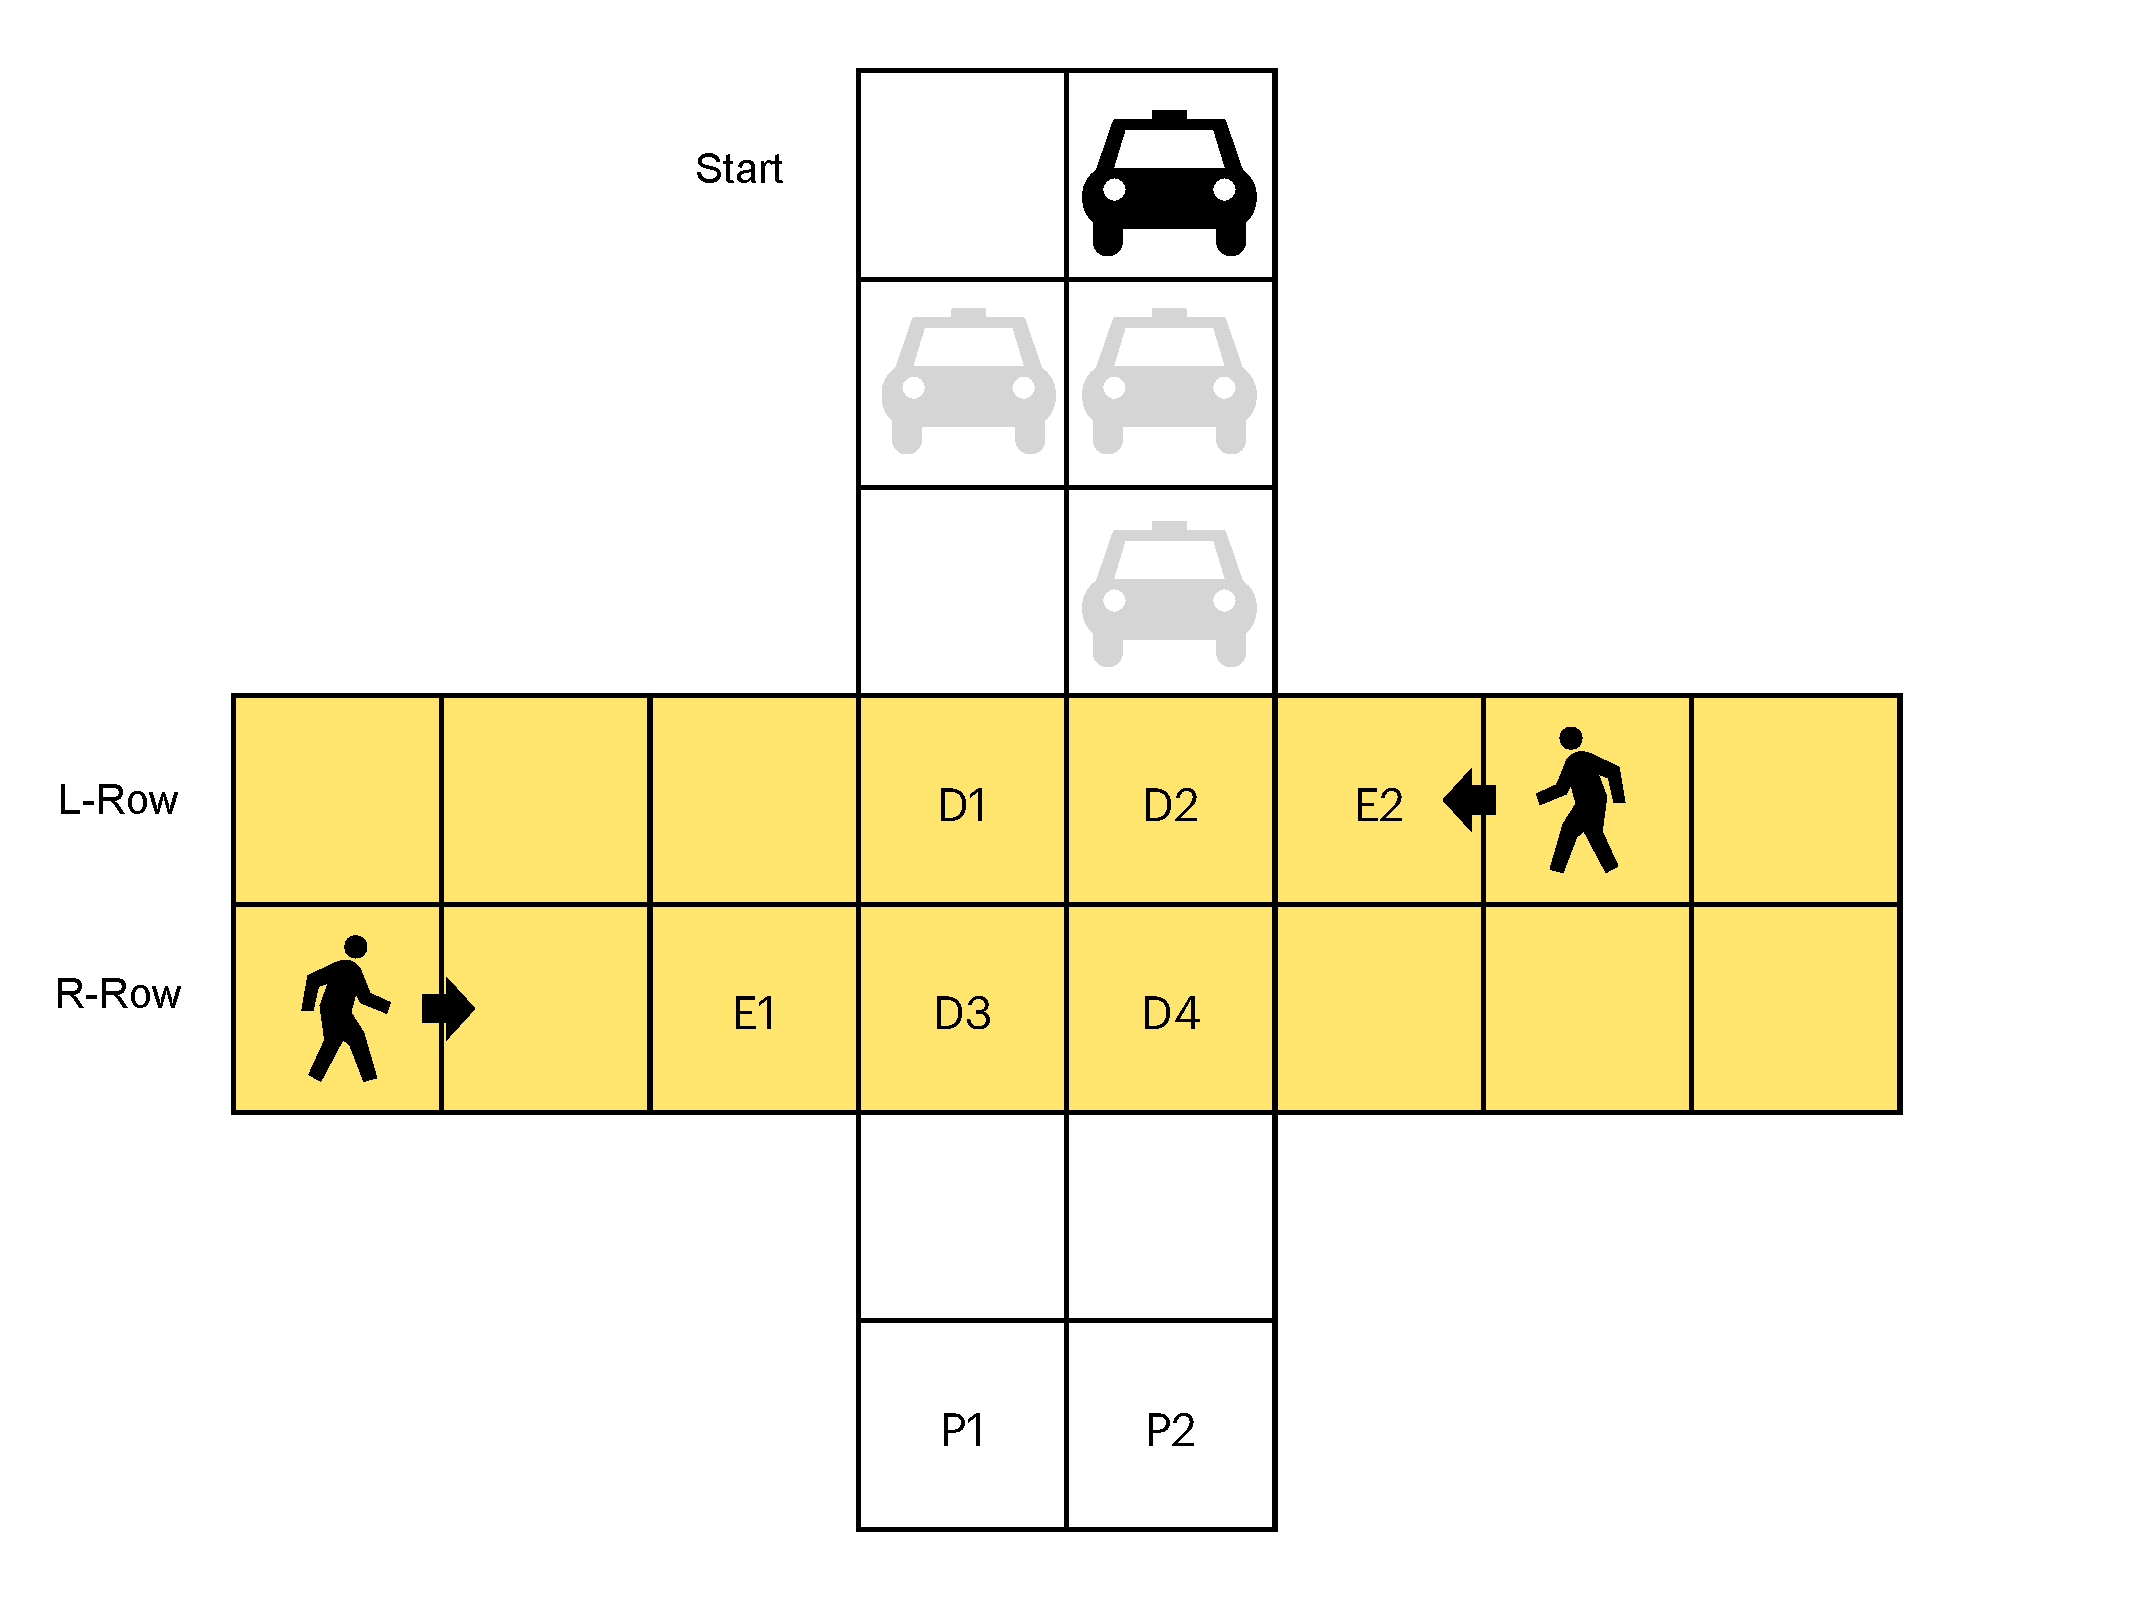
\includegraphics[width=0.8\textwidth]{rl.pdf}
    \caption{Illustration of the avoid-pedestrians-and-park problem.}
    \label{fig:my_label}
\end{figure}

Consider the safe driving problem in Figure 2. The car is the agent that you need to control. The car can only move in the two vertical lanes, and the pedestrians only in the two yellow lanes. They only make discrete moves, going from one cell to another cell in each step. Their paths intersect at the four cells in the middle, labeled as the D1-D4, where the car needs to drive cautiously, hopefully. 

The car can choose from 3 actions each time: go downward by 1 or 2 cells (i.e., corresponding to different speeds), or go sideways and downward by 1 cell (it needs to remain in the two lanes so you need to define the actions for ``sideways" reasonably). For example, suppose the car's current position is at the cell where the black car is at, its next step includes the three cells showing the grey cars. The goal of the car is to park at either the P1 or P2 cell. {\bf Important:} When the car takes the action of moving 2 cells at a time, both cells are considered occupied by the car in the next state, and the car's position is 2 cells away from the current cell. 

The two pedestrians can only move in the row that they are in following the corresponding direction indicated by the arrows, i.e., only moving left in L-Row and right in R-Row. When pedestrians go out of bounds, they just disappear (out-of-sight). 

At initialization, the two pedestrians can appear in any yellow cell in their corresponding rows. The initial position of the car is in either of the two cells at the top row (labeled as ``start"). 

Always use discount factor $\gamma=0.9$. 

In all questions, the car does not have access to the transition probabilities/rules of the environment and can only optimize its behavior through experience, i.e., following the setting of Q-learning. Also note that the transition can either use probabilities or deterministic rules, since the latter just means some transitions happen with probability 1. 

\begin{question}[2 Points]
Let's first assume that there are no pedestrians in sight or they are outside the D cells and don't move, so the car does not need to consider pedestrians. 

Roughly describe the definition of an MDP for the car agent that aims to achieve the goal of ``reaching P1 or P2 as quickly as possible" which means it should try to reach the goal cells with the least possible number of time steps. By roughly describing, we mean just explain in words the design of each component (states, actions, rewards, transitions, etc.) of the MDP, and there is no need to fully list everything in each component. 
\end{question}

\begin{question}[2 Points]
Perform Q-learning to find the optimal policy for the car for the MDP you defined in the previous question. In the answer pdf, show the Q values for the car at the cell labeled as D1, for each action that is available to the car at that position (again, assume there is no pedestrian). Since there are three actions possible there, you should show three $Q(s,a)$ values. 
\end{question}

\begin{question}[2 Points]
Now consider the two pedestrians, and assume that they can only move forward 1 cell at a time, in the specified directions. Roughly describe the definition of a new MDP that gives a large penalty and terminate the trajectory when the car hits pedestrians, i.e., when the car and any of the two pedestrians occupy the same cells at the same time. Again, when the car moves 2 cells in one step, both cells that it passes through are considered occupied. The goal of the car in this new MDP is still to reach P1 or P2 with the least amount of steps. 
\end{question}

\begin{question}[2 Points]
 Perform Q-learning for this new MDP with pedestrians that you defined in the previous question. Now you should see that the Q-values of the car depends on the positions of the pedestrians. In the answer pdf, show the Q-values for the car at the cell labeled as D1 when the R-Row pedestrian is at E1 and the L-Row pedestrian is at E2, for each action that is available to the car at that position. (If these positions correspond to multiple states in your definition, then just show the Q-values for all those states.) 
\end{question}

\begin{question}[Extra 1 Point]
Now let's change the transition in the MDP to also allow the pedestrians to move either 1 or 2 cells ahead each time, with 50\% chance for each option. When a pedestrian moves 2 cells ahead, both cells are considered occupied as well. 

The car can still only observe the current position of the pedestrian, and you shouldn't change any other part of the MDP (the change in the pedestrian behavior only affects the transition function in the environment, which is not known to the car). 

Show a trajectory of the car (i.e., list a sequence of states of the car) that starts from some initial state, and follows the optimal actions obtained by Q-learning in the previous question (i.e., learned in the previous MDP where pedestrians only move 1 cell each time), and now it collides with a pedestrian at some state in the trajectory. 

This shows the common problem of RL named ``distribution drift." The easiest way to find such problematic trajectories is to think about how the car should behave according to the previous MDP, and place the pedestrians in cells that may challenge those trained behaviors. This is also called ``adversarial attack" on the RL agent. 
\end{question}

\begin{question}[Extra 1 Point]
 Perform Q-Learning again for the car for the new MDP you defined in the previous question. Find one state of the car, where the $Q$-values of its actions have now become different from those in the MDP in Question 8. In your answer pdf, show the difference in the Q-values of the car at this state for the MDP in Question 8 and in Question 10. 
\end{question}


\section{Function Approximation in RL (No Implementation)}

\begin{question}[3 Points + 2 Extra Points]
Consider the following MDP: $S=\{s_0,s_1,s_2,s_3\}$, $A=\{a_1,a_2,a_3\}$. The transition probabilities are $P(s_1|s_0,a_1)=0.5$, $P(s_2|s_0,a_1)=0.5$, $P(s_2|s_0,a_2)=1$, $P(s_3|s_0,a_3)=1$, and all other combinations have probability 0. (So $s_1,s_2,s_3$ are terminal states.) Let the discount factor be $\gamma = 0.5$.

Suppose we want to represent the $Q$-value function as a linear function
\begin{equation}\label{q}
Q(s,a)=\alpha s + \beta a
\end{equation}
where $\alpha,\beta\in \mathbb{R}$ are the weight parameters that can be arbitrary chosen. When evaluating the function, we fix the encoding for the states and actions as $s_i=i+1$ and $a_i=i$ (e.g., $s_0=1$ and $a_1=1$). For instance, if $\alpha=2$ and $\beta=3$, then plugging them in with the encoding for the state and action we have $Q(s_0,a_1)=2\cdot 1+3\cdot 1=5$. 
\begin{enumerate}
    \item (1 Point) Draw a graph representation of the MDP (similar to Slide 13 for the chapter). 
    \item (2 Points) Design a reward function such that the linear Q function in (\ref{q}) can correctly represent all Q values at $s_0$ (you need to calculate the $Q$ values under the reward function you designed first). Show both the reward function and the corresponding linear $Q$-value function. 
    \item (1 Extra Point) Design a reward function such that the linear Q function does not work. Namely, the function in (\ref{q}) can not represent all Q values at $s_0$ for any choice of $\alpha$ and $\beta$ (i.e. the difference between the function value and the true Q value is always large for some inputs, regardless of what $\alpha,\beta$ are.). Explain the reasoning. 
    \item (1 Extra Point) Take the reward function you designed for the previous question (which fails to be captured by the linear function) and design a different function approximation scheme (different from (\ref{q})), such that all Q-values at $s_0$ can now be correctly represented. 
\end{enumerate}
Note that for all these questions we are only asking the function representation to capture the Q values at state $s_0$, i.e., it does not need to work for the other states (in general it should, just to simplify things here). 

I hope these questions make you think about the complications that using function approximators can introduce and why expressive nonlinear function approximators such as neural networks are necessary. 
\end{question}





\end{document}